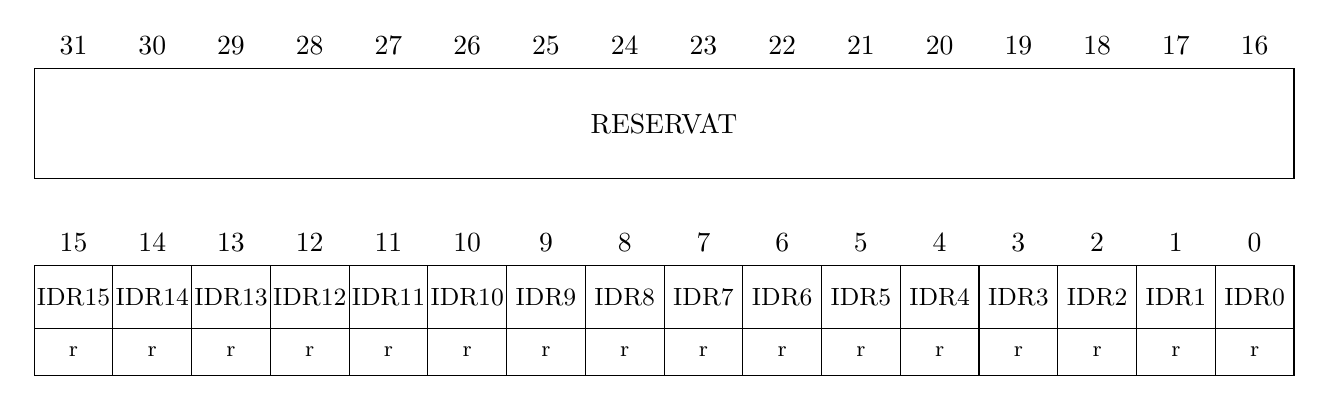
\begin{tikzpicture}
    % Numbering
    \foreach \i in {16,...,31}
    {\node[above] at(15.5+16-\i, 3.35) {\i};}

    \foreach \i in {0,...,15}
    {\node[above] at(15.5-\i, 0.85) {\i};}

    \draw[] (0, 1.9) rectangle ++(16, 1.4);
    \node[] at (8, 2.6) {RESERVAT}; 
    
    % Registre 15 - 0
    \foreach \i in {0,...,15}
    {\node[] at(15.5-\i, 0.4) {\small IDR\i};}
    \foreach \i in {0,...,15}
    {\draw[] (\i, 0) rectangle ++(1, 0.8);}
    \foreach \i in {0,...,15}
    {\draw[] (\i, -0.6) rectangle ++(1, 0.6);}
    \foreach \i in {0,...,15}
    {\node[] at(0.5+\i, -0.3) {\footnotesize r};}
\end{tikzpicture}